\section{Zielsetzung}
\label{sec:Zielsetzung}

\section{Theorie}
\label{sec:Theorie}

% Vorschlag für den Beginn, damit nicht andauernd zitiert werden muss.
Die folgende theoretische Beschreibung von ... ist aus den Quellen
\cite{anleitung} und \cite{eichler} entnommen.

\begin{figure}
  \centering
  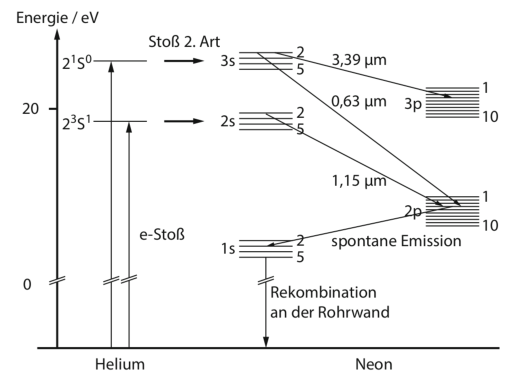
\includegraphics[height=8cm]{content/HeNe.pdf}
  \caption{Schematische Darstellung der Übergänge zur stimulierten
  Emission eines HeNe-Lasers \cite[68]{eichler}.}
  \label{fig:HeNe}
\end{figure}

\begin{figure}
  \centering
  \includegraphics[height=8cm]{build/stabilitaet.pdf}
  \caption{Darstellung der Stabilitätsparameter in Abhängigkeit der
  Resonatorlänge $L$.}
  \label{fig:Stabilität}
\end{figure}

% \subsection{Unterkapitel}
% \label{sec:UnterKapitel}

% \begin{equation}
% Für Formeln
%   \label{eqn:Formel}
% \end{equation}
